% Options for packages loaded elsewhere
\PassOptionsToPackage{unicode}{hyperref}
\PassOptionsToPackage{hyphens}{url}
\PassOptionsToPackage{dvipsnames,svgnames,x11names}{xcolor}
%
\documentclass[
]{article}
\usepackage{amsmath,amssymb}
\usepackage{iftex}
\ifPDFTeX
  \usepackage[T1]{fontenc}
  \usepackage[utf8]{inputenc}
  \usepackage{textcomp} % provide euro and other symbols
\else % if luatex or xetex
  \usepackage{unicode-math} % this also loads fontspec
  \defaultfontfeatures{Scale=MatchLowercase}
  \defaultfontfeatures[\rmfamily]{Ligatures=TeX,Scale=1}
\fi
\usepackage{lmodern}
\ifPDFTeX\else
  % xetex/luatex font selection
\fi
% Use upquote if available, for straight quotes in verbatim environments
\IfFileExists{upquote.sty}{\usepackage{upquote}}{}
\IfFileExists{microtype.sty}{% use microtype if available
  \usepackage[]{microtype}
  \UseMicrotypeSet[protrusion]{basicmath} % disable protrusion for tt fonts
}{}
\makeatletter
\@ifundefined{KOMAClassName}{% if non-KOMA class
  \IfFileExists{parskip.sty}{%
    \usepackage{parskip}
  }{% else
    \setlength{\parindent}{0pt}
    \setlength{\parskip}{6pt plus 2pt minus 1pt}}
}{% if KOMA class
  \KOMAoptions{parskip=half}}
\makeatother
\usepackage{xcolor}
\usepackage[margin=1in]{geometry}
\usepackage{color}
\usepackage{fancyvrb}
\newcommand{\VerbBar}{|}
\newcommand{\VERB}{\Verb[commandchars=\\\{\}]}
\DefineVerbatimEnvironment{Highlighting}{Verbatim}{commandchars=\\\{\}}
% Add ',fontsize=\small' for more characters per line
\usepackage{framed}
\definecolor{shadecolor}{RGB}{248,248,248}
\newenvironment{Shaded}{\begin{snugshade}}{\end{snugshade}}
\newcommand{\AlertTok}[1]{\textcolor[rgb]{0.94,0.16,0.16}{#1}}
\newcommand{\AnnotationTok}[1]{\textcolor[rgb]{0.56,0.35,0.01}{\textbf{\textit{#1}}}}
\newcommand{\AttributeTok}[1]{\textcolor[rgb]{0.13,0.29,0.53}{#1}}
\newcommand{\BaseNTok}[1]{\textcolor[rgb]{0.00,0.00,0.81}{#1}}
\newcommand{\BuiltInTok}[1]{#1}
\newcommand{\CharTok}[1]{\textcolor[rgb]{0.31,0.60,0.02}{#1}}
\newcommand{\CommentTok}[1]{\textcolor[rgb]{0.56,0.35,0.01}{\textit{#1}}}
\newcommand{\CommentVarTok}[1]{\textcolor[rgb]{0.56,0.35,0.01}{\textbf{\textit{#1}}}}
\newcommand{\ConstantTok}[1]{\textcolor[rgb]{0.56,0.35,0.01}{#1}}
\newcommand{\ControlFlowTok}[1]{\textcolor[rgb]{0.13,0.29,0.53}{\textbf{#1}}}
\newcommand{\DataTypeTok}[1]{\textcolor[rgb]{0.13,0.29,0.53}{#1}}
\newcommand{\DecValTok}[1]{\textcolor[rgb]{0.00,0.00,0.81}{#1}}
\newcommand{\DocumentationTok}[1]{\textcolor[rgb]{0.56,0.35,0.01}{\textbf{\textit{#1}}}}
\newcommand{\ErrorTok}[1]{\textcolor[rgb]{0.64,0.00,0.00}{\textbf{#1}}}
\newcommand{\ExtensionTok}[1]{#1}
\newcommand{\FloatTok}[1]{\textcolor[rgb]{0.00,0.00,0.81}{#1}}
\newcommand{\FunctionTok}[1]{\textcolor[rgb]{0.13,0.29,0.53}{\textbf{#1}}}
\newcommand{\ImportTok}[1]{#1}
\newcommand{\InformationTok}[1]{\textcolor[rgb]{0.56,0.35,0.01}{\textbf{\textit{#1}}}}
\newcommand{\KeywordTok}[1]{\textcolor[rgb]{0.13,0.29,0.53}{\textbf{#1}}}
\newcommand{\NormalTok}[1]{#1}
\newcommand{\OperatorTok}[1]{\textcolor[rgb]{0.81,0.36,0.00}{\textbf{#1}}}
\newcommand{\OtherTok}[1]{\textcolor[rgb]{0.56,0.35,0.01}{#1}}
\newcommand{\PreprocessorTok}[1]{\textcolor[rgb]{0.56,0.35,0.01}{\textit{#1}}}
\newcommand{\RegionMarkerTok}[1]{#1}
\newcommand{\SpecialCharTok}[1]{\textcolor[rgb]{0.81,0.36,0.00}{\textbf{#1}}}
\newcommand{\SpecialStringTok}[1]{\textcolor[rgb]{0.31,0.60,0.02}{#1}}
\newcommand{\StringTok}[1]{\textcolor[rgb]{0.31,0.60,0.02}{#1}}
\newcommand{\VariableTok}[1]{\textcolor[rgb]{0.00,0.00,0.00}{#1}}
\newcommand{\VerbatimStringTok}[1]{\textcolor[rgb]{0.31,0.60,0.02}{#1}}
\newcommand{\WarningTok}[1]{\textcolor[rgb]{0.56,0.35,0.01}{\textbf{\textit{#1}}}}
\usepackage{longtable,booktabs,array}
\usepackage{calc} % for calculating minipage widths
% Correct order of tables after \paragraph or \subparagraph
\usepackage{etoolbox}
\makeatletter
\patchcmd\longtable{\par}{\if@noskipsec\mbox{}\fi\par}{}{}
\makeatother
% Allow footnotes in longtable head/foot
\IfFileExists{footnotehyper.sty}{\usepackage{footnotehyper}}{\usepackage{footnote}}
\makesavenoteenv{longtable}
\usepackage{graphicx}
\makeatletter
\def\maxwidth{\ifdim\Gin@nat@width>\linewidth\linewidth\else\Gin@nat@width\fi}
\def\maxheight{\ifdim\Gin@nat@height>\textheight\textheight\else\Gin@nat@height\fi}
\makeatother
% Scale images if necessary, so that they will not overflow the page
% margins by default, and it is still possible to overwrite the defaults
% using explicit options in \includegraphics[width, height, ...]{}
\setkeys{Gin}{width=\maxwidth,height=\maxheight,keepaspectratio}
% Set default figure placement to htbp
\makeatletter
\def\fps@figure{htbp}
\makeatother
\setlength{\emergencystretch}{3em} % prevent overfull lines
\providecommand{\tightlist}{%
  \setlength{\itemsep}{0pt}\setlength{\parskip}{0pt}}
\setcounter{secnumdepth}{-\maxdimen} % remove section numbering
\ifLuaTeX
  \usepackage{selnolig}  % disable illegal ligatures
\fi
\IfFileExists{bookmark.sty}{\usepackage{bookmark}}{\usepackage{hyperref}}
\IfFileExists{xurl.sty}{\usepackage{xurl}}{} % add URL line breaks if available
\urlstyle{same}
\hypersetup{
  pdftitle={STAT 847: Analysis Assignment 2},
  colorlinks=true,
  linkcolor={Maroon},
  filecolor={Maroon},
  citecolor={Blue},
  urlcolor={blue},
  pdfcreator={LaTeX via pandoc}}

\title{STAT 847: Analysis Assignment 2}
\author{}
\date{\vspace{-2.5em}}

\begin{document}
\maketitle

This dataset contains all five phenotypes and the first 10,000 SNPs from
a Genome-Wide Association Study of the species Arabidopsis thaliana, a
plant.

\begin{longtable}[]{@{}
  >{\raggedright\arraybackslash}p{(\columnwidth - 2\tabcolsep) * \real{0.2222}}
  >{\raggedright\arraybackslash}p{(\columnwidth - 2\tabcolsep) * \real{0.7778}}@{}}
\toprule\noalign{}
\begin{minipage}[b]{\linewidth}\raggedright
Variable
\end{minipage} & \begin{minipage}[b]{\linewidth}\raggedright
Description
\end{minipage} \\
\midrule\noalign{}
\endhead
\bottomrule\noalign{}
\endlastfoot
See: &
\url{https://easygwas.biochem.mpg.de/data/public/dataset/view/42/} \\
Perimeter\_Growth & The response variable \\
SNP\_ABCD & The explanatory variable, gene number ABCD \\
& \\
\end{longtable}

Note: These have been coded into 0, 1, 2, or 3, so, while treating these
continuous variables isn't the correct thing to do, we're going to do it
anyways because a our methods will be able to pick out some of the
important genes even with the mispecification.

Use the following code to load and split the data

\begin{Shaded}
\begin{Highlighting}[]
\FunctionTok{library}\NormalTok{(randomForest)}
\end{Highlighting}
\end{Shaded}

\begin{verbatim}
## randomForest 4.7-1.1
\end{verbatim}

\begin{verbatim}
## Type rfNews() to see new features/changes/bug fixes.
\end{verbatim}

\begin{Shaded}
\begin{Highlighting}[]
\NormalTok{dat }\OtherTok{=} \FunctionTok{read.csv}\NormalTok{(}\StringTok{"/Users/andrew/Downloads/UW courses/STAT 847/Analysis 2/F1{-}Hybrids\_Pheno\_10000genes.csv"}\NormalTok{)}

\NormalTok{genes }\OtherTok{=}\NormalTok{ dat[,}\DecValTok{9}\SpecialCharTok{:}\DecValTok{10008}\NormalTok{]}
\NormalTok{pheno }\OtherTok{=}\NormalTok{ dat[,}\DecValTok{1}\SpecialCharTok{:}\DecValTok{8}\NormalTok{]}
\NormalTok{dat }\OtherTok{=} \ConstantTok{NULL}
\end{Highlighting}
\end{Shaded}

\vspace{2cm}

\begin{enumerate}
\def\labelenumi{\arabic{enumi}.}
\tightlist
\item
  (4 points) Using the \texttt{randomForest} function in
  \texttt{library(randomForest)}, make five random forests, each one
  using one of the phenotype variable \texttt{Perimeter\_Growth} as a
  response y variable. The forest should use all 10,000 of the gene
  variables (These are the 9th, \ldots{} , 10,008th variables). Give
  your forest 500 trees, have each tree use 300 gene variables, and set
  a minimum node size of 1. Sample with replacement. Report the
  percentage of variance explained by the forest using \texttt{print()}.
\end{enumerate}

\begin{Shaded}
\begin{Highlighting}[]
\CommentTok{\# Load the required library}
\FunctionTok{library}\NormalTok{(randomForest)}

\CommentTok{\# Assuming your datasets are named pheno and gene}

\CommentTok{\# Extracting the phenotype variable Perimeter\_Growth}
\NormalTok{response\_variable }\OtherTok{\textless{}{-}}\NormalTok{ pheno}\SpecialCharTok{$}\NormalTok{Perimeter\_Growth}

\CommentTok{\# Extracting the gene variables}
\NormalTok{gene\_variables }\OtherTok{\textless{}{-}}\NormalTok{ genes}

\CommentTok{\# Number of trees in the forest}
\NormalTok{num\_trees }\OtherTok{\textless{}{-}} \DecValTok{500}

\CommentTok{\# Number of gene variables to be used in each tree}
\NormalTok{num\_gene\_variables }\OtherTok{\textless{}{-}} \DecValTok{300}

\CommentTok{\# Minimum node size}
\NormalTok{min\_node\_size }\OtherTok{\textless{}{-}} \DecValTok{1}

\CommentTok{\# Perform five random forests}
\ControlFlowTok{for}\NormalTok{ (i }\ControlFlowTok{in} \DecValTok{1}\SpecialCharTok{:}\DecValTok{5}\NormalTok{) \{}
  \CommentTok{\# Create a random forest}
\NormalTok{  rf }\OtherTok{\textless{}{-}} \FunctionTok{randomForest}\NormalTok{(}\AttributeTok{x =}\NormalTok{ gene\_variables, }\AttributeTok{y =}\NormalTok{ response\_variable, }
                     \AttributeTok{ntree =}\NormalTok{ num\_trees, }\AttributeTok{mtry =}\NormalTok{ num\_gene\_variables, }
                     \AttributeTok{nodesize =}\NormalTok{ min\_node\_size, }\AttributeTok{replace =} \ConstantTok{TRUE}\NormalTok{)}
  
  \CommentTok{\# Print the percentage of variance explained by the forest}
  \FunctionTok{print}\NormalTok{(rf)}
\NormalTok{\}}
\end{Highlighting}
\end{Shaded}

\begin{verbatim}
## 
## Call:
##  randomForest(x = gene_variables, y = response_variable, ntree = num_trees,      mtry = num_gene_variables, replace = TRUE, nodesize = min_node_size) 
##                Type of random forest: regression
##                      Number of trees: 500
## No. of variables tried at each split: 300
## 
##           Mean of squared residuals: 1.529967
##                     % Var explained: 39.43
## 
## Call:
##  randomForest(x = gene_variables, y = response_variable, ntree = num_trees,      mtry = num_gene_variables, replace = TRUE, nodesize = min_node_size) 
##                Type of random forest: regression
##                      Number of trees: 500
## No. of variables tried at each split: 300
## 
##           Mean of squared residuals: 1.553748
##                     % Var explained: 38.49
## 
## Call:
##  randomForest(x = gene_variables, y = response_variable, ntree = num_trees,      mtry = num_gene_variables, replace = TRUE, nodesize = min_node_size) 
##                Type of random forest: regression
##                      Number of trees: 500
## No. of variables tried at each split: 300
## 
##           Mean of squared residuals: 1.51938
##                     % Var explained: 39.85
## 
## Call:
##  randomForest(x = gene_variables, y = response_variable, ntree = num_trees,      mtry = num_gene_variables, replace = TRUE, nodesize = min_node_size) 
##                Type of random forest: regression
##                      Number of trees: 500
## No. of variables tried at each split: 300
## 
##           Mean of squared residuals: 1.535044
##                     % Var explained: 39.23
## 
## Call:
##  randomForest(x = gene_variables, y = response_variable, ntree = num_trees,      mtry = num_gene_variables, replace = TRUE, nodesize = min_node_size) 
##                Type of random forest: regression
##                      Number of trees: 500
## No. of variables tried at each split: 300
## 
##           Mean of squared residuals: 1.529513
##                     % Var explained: 39.45
\end{verbatim}

\vspace{2cm}

\newpage

\begin{enumerate}
\def\labelenumi{\arabic{enumi}.}
\setcounter{enumi}{1}
\tightlist
\item
  (2 points) Get a \texttt{hist()} of the \texttt{\$importance} values
  from your random forest model of perimeter growth (not the MPH). Use
  this to comment on the relative importance of some genes over others
  in determining perimeter growth. Use 100 bins for the histogram.
\end{enumerate}

\begin{Shaded}
\begin{Highlighting}[]
\CommentTok{\# Create a random forest model for perimeter growth}
\NormalTok{rf\_perimeter\_growth }\OtherTok{\textless{}{-}} \FunctionTok{randomForest}\NormalTok{(}\AttributeTok{x =}\NormalTok{ gene\_variables, }\AttributeTok{y =}\NormalTok{ pheno}\SpecialCharTok{$}\NormalTok{Perimeter\_Growth,}
                                    \AttributeTok{ntree =}\NormalTok{ num\_trees, }\AttributeTok{mtry =}\NormalTok{ num\_gene\_variables, }
                                    \AttributeTok{nodesize =}\NormalTok{ min\_node\_size, }\AttributeTok{replace =} \ConstantTok{TRUE}\NormalTok{)}

\CommentTok{\# Get the importance values from the model}
\NormalTok{importance\_values }\OtherTok{\textless{}{-}}\NormalTok{ rf\_perimeter\_growth}\SpecialCharTok{$}\NormalTok{importance}

\CommentTok{\# Plot a histogram of the importance values}
\FunctionTok{hist}\NormalTok{(importance\_values, }\AttributeTok{breaks =} \DecValTok{100}\NormalTok{, }\AttributeTok{main =} \StringTok{"Importance Values of Genes for Perimeter Growth"}\NormalTok{,}
     \AttributeTok{xlab =} \StringTok{"Importance"}\NormalTok{, }\AttributeTok{ylab =} \StringTok{"Frequency"}\NormalTok{)}
\end{Highlighting}
\end{Shaded}

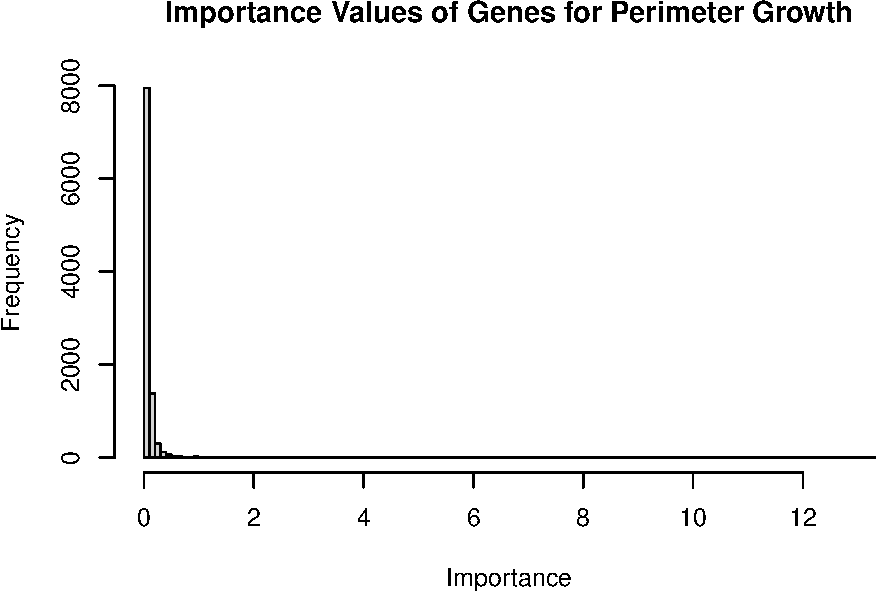
\includegraphics{STAT847_W24_Analysis2_files/figure-latex/unnamed-chunk-3-1.pdf}
\newpage

\vspace{2cm}

\begin{enumerate}
\def\labelenumi{\arabic{enumi}.}
\setcounter{enumi}{2}
\tightlist
\item
  (0 marks) Use the following code to make a new dataset that only
  includes perimeter growth and the most important 50 genetic variables
  from random forest for perimeter growth. \texttt{mod2} is the name of
  the \texttt{randomForest()} output in this case.
\end{enumerate}

\begin{Shaded}
\begin{Highlighting}[]
\CommentTok{\# mod2 is }
\CommentTok{\# Set a cutoff of the 50th most important variable}
\NormalTok{cutoff }\OtherTok{=} \FunctionTok{rev}\NormalTok{(}\FunctionTok{sort}\NormalTok{(rf\_perimeter\_growth}\SpecialCharTok{$}\NormalTok{importance))[}\DecValTok{50}\NormalTok{]}

\CommentTok{\# Keep only those 50 variables}
\NormalTok{idx }\OtherTok{=} \FunctionTok{which}\NormalTok{(rf\_perimeter\_growth}\SpecialCharTok{$}\NormalTok{importance }\SpecialCharTok{\textgreater{}=}\NormalTok{ cutoff)}
\NormalTok{genes\_imp }\OtherTok{=}\NormalTok{ genes[,idx]}

\NormalTok{dat\_imp }\OtherTok{=} \FunctionTok{cbind}\NormalTok{(pheno}\SpecialCharTok{$}\NormalTok{Perimeter\_Growth, genes\_imp)}
\FunctionTok{names}\NormalTok{(dat\_imp)[}\DecValTok{1}\NormalTok{] }\OtherTok{=} \StringTok{"Perimeter\_Growth"}
\end{Highlighting}
\end{Shaded}

\vspace{2cm}

\newpage
4

. (4 points) Using \texttt{rpart}, and this new dataset
\texttt{dat\_imp} (or \texttt{genes\_imp}) of the 50 most important
variables for perimeter growth, create a single regression tree of
perimeter growth. Plot the tree with \texttt{prp} in the
\texttt{rpart.plot} package.

\begin{Shaded}
\begin{Highlighting}[]
\CommentTok{\# Load the required libraries}
\FunctionTok{library}\NormalTok{(rpart)}
\FunctionTok{library}\NormalTok{(rpart.plot)}

\CommentTok{\# Create a regression tree using rpart}
\NormalTok{tree\_model }\OtherTok{\textless{}{-}} \FunctionTok{rpart}\NormalTok{(Perimeter\_Growth }\SpecialCharTok{\textasciitilde{}}\NormalTok{ ., }\AttributeTok{data =}\NormalTok{ dat\_imp)}

\CommentTok{\# Plot the tree using prp}
\FunctionTok{prp}\NormalTok{(tree\_model, }\AttributeTok{type =} \DecValTok{2}\NormalTok{, }\AttributeTok{extra =} \DecValTok{1}\NormalTok{, }\AttributeTok{branch =} \DecValTok{1}\NormalTok{, }\AttributeTok{varlen =} \DecValTok{0}\NormalTok{, }\AttributeTok{yesno =} \DecValTok{2}\NormalTok{,}
    \AttributeTok{box.palette =} \FunctionTok{c}\NormalTok{(}\StringTok{"skyblue"}\NormalTok{, }\StringTok{"pink"}\NormalTok{), }\AttributeTok{fallen.leaves =} \ConstantTok{TRUE}\NormalTok{)}
\end{Highlighting}
\end{Shaded}

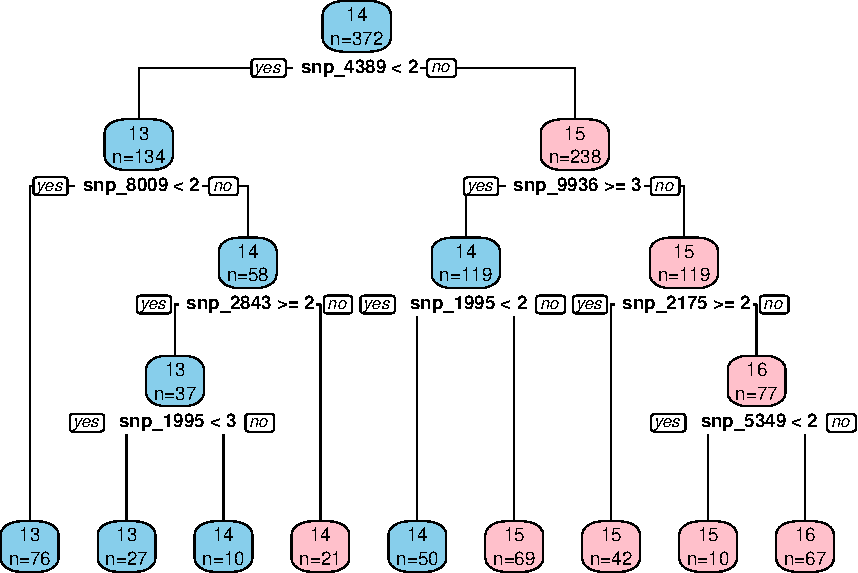
\includegraphics{STAT847_W24_Analysis2_files/figure-latex/unnamed-chunk-5-1.pdf}

\vspace{2cm}
\newpage

\begin{enumerate}
\def\labelenumi{\arabic{enumi}.}
\setcounter{enumi}{4}
\tightlist
\item
  (4 marks) Using \texttt{regsubsets} in the \texttt{leaps} package, and
  the new dataset \texttt{dat\_imp} (or \texttt{genes\_imp}), use best
  subsets regression with the Adjusted R-squared criterion. Report the
  variables of the best model, their coefficients, and the adjusted
  r-squared of the model.
\end{enumerate}

Hints:

To get the adjusted r-squared values, use \texttt{summary(regsubsets())}

To get a particular model, see
\url{https://stats.stackexchange.com/questions/193204/picking-a-particular-model-from-regsubsets}

\begin{Shaded}
\begin{Highlighting}[]
\CommentTok{\# Load the required libraries}
\FunctionTok{library}\NormalTok{(leaps)}
\FunctionTok{library}\NormalTok{(caret)}
\end{Highlighting}
\end{Shaded}

\begin{verbatim}
## Loading required package: ggplot2
\end{verbatim}

\begin{verbatim}
## 
## Attaching package: 'ggplot2'
\end{verbatim}

\begin{verbatim}
## The following object is masked from 'package:randomForest':
## 
##     margin
\end{verbatim}

\begin{verbatim}
## Loading required package: lattice
\end{verbatim}

\begin{Shaded}
\begin{Highlighting}[]
\CommentTok{\# Check for multicollinearity}
\NormalTok{cor\_dat\_imp }\OtherTok{\textless{}{-}} \FunctionTok{cor}\NormalTok{(dat\_imp[,}\SpecialCharTok{{-}}\DecValTok{1}\NormalTok{]) }\CommentTok{\# Compute correlation matrix, excluding the response variable}
\NormalTok{highly\_correlated }\OtherTok{\textless{}{-}} \FunctionTok{findCorrelation}\NormalTok{(cor\_dat\_imp, }\AttributeTok{cutoff =} \FloatTok{0.8}\NormalTok{) }\CommentTok{\# Find highly correlated variables}

\CommentTok{\# Remove highly correlated variables}
\NormalTok{dat\_imp\_filtered }\OtherTok{\textless{}{-}}\NormalTok{ dat\_imp[, }\SpecialCharTok{{-}}\FunctionTok{c}\NormalTok{(highly\_correlated }\SpecialCharTok{+} \DecValTok{1}\NormalTok{)] }\CommentTok{\# +1 to account for removing the response variable column}

\CommentTok{\# Perform best subsets regression}
\NormalTok{best\_model }\OtherTok{\textless{}{-}} \FunctionTok{regsubsets}\NormalTok{(Perimeter\_Growth }\SpecialCharTok{\textasciitilde{}}\NormalTok{ ., }\AttributeTok{data =}\NormalTok{ dat\_imp\_filtered, }\AttributeTok{method =} \StringTok{"exhaustive"}\NormalTok{)}

\CommentTok{\# Get the summary of the best model}
\NormalTok{summary\_best\_model }\OtherTok{\textless{}{-}} \FunctionTok{summary}\NormalTok{(best\_model)}

\CommentTok{\# Find the index of the best model based on adjusted R{-}squared}
\NormalTok{best\_model\_index }\OtherTok{\textless{}{-}} \FunctionTok{which.max}\NormalTok{(summary\_best\_model}\SpecialCharTok{$}\NormalTok{adjr2)}

\CommentTok{\# Get the best model}
\NormalTok{best\_model\_variables }\OtherTok{\textless{}{-}} \FunctionTok{names}\NormalTok{(}\FunctionTok{which}\NormalTok{(}\FunctionTok{coef}\NormalTok{(best\_model, }\AttributeTok{id =}\NormalTok{ best\_model\_index) }\SpecialCharTok{!=} \DecValTok{0}\NormalTok{))}
\NormalTok{best\_model\_coefficients }\OtherTok{\textless{}{-}} \FunctionTok{coef}\NormalTok{(best\_model, }\AttributeTok{id =}\NormalTok{ best\_model\_index)}
\NormalTok{adjusted\_r\_squared }\OtherTok{\textless{}{-}}\NormalTok{ summary\_best\_model}\SpecialCharTok{$}\NormalTok{adjr2[best\_model\_index]}

\CommentTok{\# Report the variables of the best model}
\FunctionTok{cat}\NormalTok{(}\StringTok{"Variables of the best model:"}\NormalTok{, }\StringTok{"}\SpecialCharTok{\textbackslash{}n}\StringTok{"}\NormalTok{)}
\end{Highlighting}
\end{Shaded}

\begin{verbatim}
## Variables of the best model:
\end{verbatim}

\begin{Shaded}
\begin{Highlighting}[]
\FunctionTok{print}\NormalTok{(best\_model\_variables)}
\end{Highlighting}
\end{Shaded}

\begin{verbatim}
## [1] "(Intercept)" "snp_898"     "snp_1995"    "snp_2175"    "snp_2843"   
## [6] "snp_2864"    "snp_4390"    "snp_6120"    "snp_9934"
\end{verbatim}

\begin{Shaded}
\begin{Highlighting}[]
\CommentTok{\# Report the coefficients of the best model}
\FunctionTok{cat}\NormalTok{(}\StringTok{"}\SpecialCharTok{\textbackslash{}n}\StringTok{Coefficients of the best model:"}\NormalTok{, }\StringTok{"}\SpecialCharTok{\textbackslash{}n}\StringTok{"}\NormalTok{)}
\end{Highlighting}
\end{Shaded}

\begin{verbatim}
## 
## Coefficients of the best model:
\end{verbatim}

\begin{Shaded}
\begin{Highlighting}[]
\FunctionTok{print}\NormalTok{(best\_model\_coefficients)}
\end{Highlighting}
\end{Shaded}

\begin{verbatim}
## (Intercept)     snp_898    snp_1995    snp_2175    snp_2843    snp_2864 
##  14.0692276  -0.3145819   0.2905138  -0.1652086  -0.2777866   0.3656500 
##    snp_4390    snp_6120    snp_9934 
##   0.2589616   0.3103362  -0.3014517
\end{verbatim}

\begin{Shaded}
\begin{Highlighting}[]
\CommentTok{\# Report the adjusted R{-}squared of the best model}
\FunctionTok{cat}\NormalTok{(}\StringTok{"}\SpecialCharTok{\textbackslash{}n}\StringTok{Adjusted R{-}squared of the best model:"}\NormalTok{, }\StringTok{"}\SpecialCharTok{\textbackslash{}n}\StringTok{"}\NormalTok{)}
\end{Highlighting}
\end{Shaded}

\begin{verbatim}
## 
## Adjusted R-squared of the best model:
\end{verbatim}

\begin{Shaded}
\begin{Highlighting}[]
\FunctionTok{print}\NormalTok{(adjusted\_r\_squared)}
\end{Highlighting}
\end{Shaded}

\begin{verbatim}
## [1] 0.4714407
\end{verbatim}

\newpage
\vspace{2cm}

\begin{enumerate}
\def\labelenumi{\arabic{enumi}.}
\setcounter{enumi}{5}
\tightlist
\item
  (4 marks) Run a PCA on the 50 important variables in
  \texttt{genes\_imp}. Report the total (cumulative) variance explained
  by the first 10 principal components. Plot a scree plot.
\end{enumerate}

\begin{Shaded}
\begin{Highlighting}[]
\CommentTok{\# Perform PCA on the 50 important variables in genes\_imp}
\NormalTok{pca\_result }\OtherTok{\textless{}{-}} \FunctionTok{prcomp}\NormalTok{(genes\_imp, }\AttributeTok{scale. =} \ConstantTok{TRUE}\NormalTok{)}

\CommentTok{\# Extract the variance explained by each principal component}
\NormalTok{variance\_explained }\OtherTok{\textless{}{-}}\NormalTok{ pca\_result}\SpecialCharTok{$}\NormalTok{sdev}\SpecialCharTok{\^{}}\DecValTok{2}

\CommentTok{\# Calculate the cumulative variance explained}
\NormalTok{cumulative\_variance\_explained }\OtherTok{\textless{}{-}} \FunctionTok{cumsum}\NormalTok{(variance\_explained)}

\CommentTok{\# Report the total variance explained by the first 10 principal components}
\NormalTok{total\_variance\_explained\_10PCs }\OtherTok{\textless{}{-}} \FunctionTok{sum}\NormalTok{(variance\_explained[}\DecValTok{1}\SpecialCharTok{:}\DecValTok{10}\NormalTok{])}

\FunctionTok{cat}\NormalTok{(}\StringTok{"Total variance explained by the first 10 principal components:"}\NormalTok{, }\StringTok{"}\SpecialCharTok{\textbackslash{}n}\StringTok{"}\NormalTok{)}
\end{Highlighting}
\end{Shaded}

\begin{verbatim}
## Total variance explained by the first 10 principal components:
\end{verbatim}

\begin{Shaded}
\begin{Highlighting}[]
\FunctionTok{print}\NormalTok{(total\_variance\_explained\_10PCs)}
\end{Highlighting}
\end{Shaded}

\begin{verbatim}
## [1] 43.61051
\end{verbatim}

\begin{Shaded}
\begin{Highlighting}[]
\CommentTok{\# Plot a scree plot}
\FunctionTok{plot}\NormalTok{(}\DecValTok{1}\SpecialCharTok{:}\FunctionTok{length}\NormalTok{(variance\_explained), variance\_explained, }\AttributeTok{type =} \StringTok{"b"}\NormalTok{, }
     \AttributeTok{main =} \StringTok{"Scree Plot"}\NormalTok{, }\AttributeTok{xlab =} \StringTok{"Principal Component"}\NormalTok{, }\AttributeTok{ylab =} \StringTok{"Variance Explained"}\NormalTok{)}
\end{Highlighting}
\end{Shaded}

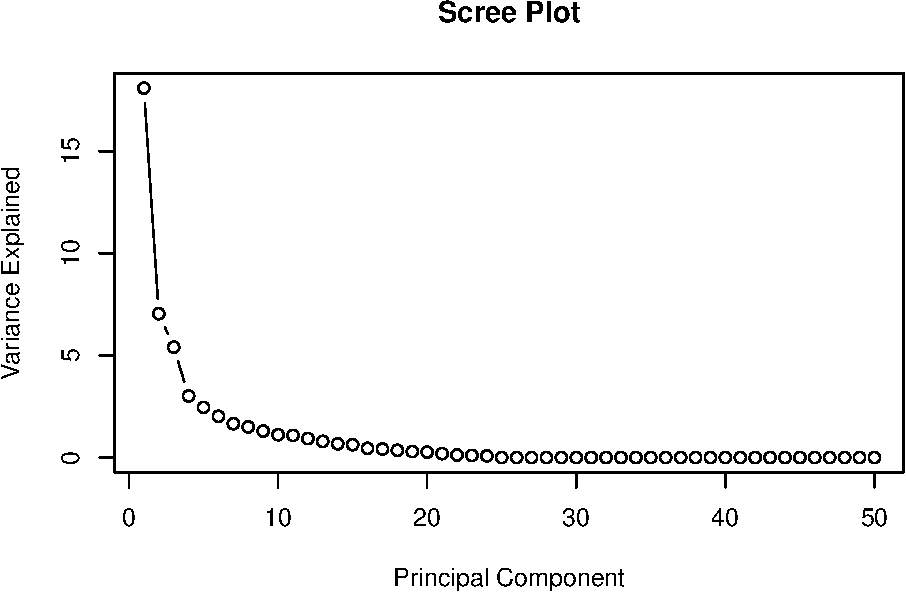
\includegraphics{STAT847_W24_Analysis2_files/figure-latex/unnamed-chunk-7-1.pdf}

\newpage
\vspace{2cm}

\begin{enumerate}
\def\labelenumi{\arabic{enumi}.}
\setcounter{enumi}{6}
\tightlist
\item
  (4 marks) Build a linear model of the response variable
  \texttt{Perimeter\_Growth} using the first ten PCA dimensions from the
  previous question, and nothing else. Report the
  \texttt{summary(lm())}. Comment on the difference between this model's
  adjusted R-squared and the
\end{enumerate}

The adjusted r-squared values for the top 10 PCs and the best subsets
model are about the same.

\begin{Shaded}
\begin{Highlighting}[]
\CommentTok{\# Extract the first ten PCA dimensions}
\NormalTok{pca\_dimensions }\OtherTok{\textless{}{-}} \FunctionTok{as.data.frame}\NormalTok{(pca\_result}\SpecialCharTok{$}\NormalTok{x[, }\DecValTok{1}\SpecialCharTok{:}\DecValTok{10}\NormalTok{])}

\CommentTok{\# Build a linear model using the first ten PCA dimensions}
\NormalTok{lm\_pca }\OtherTok{\textless{}{-}} \FunctionTok{lm}\NormalTok{(pheno}\SpecialCharTok{$}\NormalTok{Perimeter\_Growth }\SpecialCharTok{\textasciitilde{}}\NormalTok{ ., }\AttributeTok{data =}\NormalTok{ pca\_dimensions)}

\CommentTok{\# Report the summary of the linear model}
\NormalTok{summary\_lm\_pca }\OtherTok{\textless{}{-}} \FunctionTok{summary}\NormalTok{(lm\_pca)}
\FunctionTok{print}\NormalTok{(summary\_lm\_pca)}
\end{Highlighting}
\end{Shaded}

\begin{verbatim}
## 
## Call:
## lm(formula = pheno$Perimeter_Growth ~ ., data = pca_dimensions)
## 
## Residuals:
##     Min      1Q  Median      3Q     Max 
## -4.9458 -0.7375  0.0484  0.6556  4.1716 
## 
## Coefficients:
##              Estimate Std. Error t value Pr(>|t|)    
## (Intercept) 14.314808   0.059412 240.942  < 2e-16 ***
## PC1          0.224153   0.013987  16.026  < 2e-16 ***
## PC2          0.191866   0.022415   8.560  3.3e-16 ***
## PC3          0.003432   0.025587   0.134   0.8934    
## PC4          0.072734   0.034260   2.123   0.0344 *  
## PC5         -0.037789   0.037966  -0.995   0.3202    
## PC6          0.087878   0.041817   2.101   0.0363 *  
## PC7          0.116248   0.046204   2.516   0.0123 *  
## PC8          0.036525   0.048555   0.752   0.4524    
## PC9          0.131221   0.052252   2.511   0.0125 *  
## PC10         0.066833   0.056228   1.189   0.2354    
## ---
## Signif. codes:  0 '***' 0.001 '**' 0.01 '*' 0.05 '.' 0.1 ' ' 1
## 
## Residual standard error: 1.146 on 361 degrees of freedom
## Multiple R-squared:  0.4956, Adjusted R-squared:  0.4816 
## F-statistic: 35.46 on 10 and 361 DF,  p-value: < 2.2e-16
\end{verbatim}

\newpage

\vspace{2cm}

\begin{enumerate}
\def\labelenumi{\arabic{enumi}.}
\setcounter{enumi}{7}
\tightlist
\item
  (4 marks) Describe briefly one advantage and one disadvantage of the
  PCA-based model over the best subsets model. (There are several
  correct answers, but only the first two will be marked).
\end{enumerate}

One advantage of the PCA-based model over the best subsets model is its
ability to handle multicollinearity effectively. PCA reduces the
dimensionality of the data by transforming the original variables into a
new set of uncorrelated variables (principal components), which can help
mitigate multicollinearity issues present in the original data.

One disadvantage of the PCA-based model is the potential loss of
interpretability. PCA creates linear combinations of the original
variables, making it challenging to interpret the coefficients of the
principal components in terms of the original variables. This loss of
interpretability can hinder the understanding of the relationship
between the predictors and the response variable compared to models
built directly on the original variables, such as the best subsets
model.

\vspace{2cm}

\newpage

\begin{enumerate}
\def\labelenumi{\arabic{enumi}.}
\setcounter{enumi}{8}
\tightlist
\item
  (4 marks) The variance inflation factor of an explanatory variable in
  a model is a function of how collinear that variable is with the over
  explanatory variables in the model are. The higher the number, the
  more collinear and the most the variance estimates of the slopes are
  being inflated by including that variable. We can find the variable
  inflation factor with \texttt{vif(lm())}, where \texttt{vif} is found
  in the \texttt{car} package.
\end{enumerate}

Find the \texttt{vif()} of both the PCA-based model and best-subsets
model.

Report the VIFs for both models and briefly explain why the PCA-based
model has such low inflation factors (1 is the lowest possible).

\begin{Shaded}
\begin{Highlighting}[]
\CommentTok{\# Load the required library}
\FunctionTok{library}\NormalTok{(car)}
\end{Highlighting}
\end{Shaded}

\begin{verbatim}
## Loading required package: carData
\end{verbatim}

\begin{Shaded}
\begin{Highlighting}[]
\CommentTok{\# Find the VIFs for the PCA{-}based model}
\NormalTok{vif\_pca }\OtherTok{\textless{}{-}} \FunctionTok{vif}\NormalTok{(lm\_pca)}

\CommentTok{\# Find the VIFs for the best subsets model}
\CommentTok{\# Assuming \textquotesingle{}best\_model\textquotesingle{} contains the linear regression model from best subsets}
\NormalTok{vif\_best\_subsets }\OtherTok{\textless{}{-}} \FunctionTok{vif}\NormalTok{(}\FunctionTok{lm}\NormalTok{(Perimeter\_Growth }\SpecialCharTok{\textasciitilde{}}\NormalTok{ ., }\AttributeTok{data =}\NormalTok{ dat\_imp\_filtered, }\AttributeTok{method =} \StringTok{"exhaustive"}\NormalTok{))}
\end{Highlighting}
\end{Shaded}

\begin{verbatim}
## Warning in lm(Perimeter_Growth ~ ., data = dat_imp_filtered, method =
## "exhaustive"): method = 'exhaustive' is not supported. Using 'qr'
\end{verbatim}

\begin{Shaded}
\begin{Highlighting}[]
\CommentTok{\# Report the VIFs for both models}
\FunctionTok{cat}\NormalTok{(}\StringTok{"VIFs for the PCA{-}based model:"}\NormalTok{, }\StringTok{"}\SpecialCharTok{\textbackslash{}n}\StringTok{"}\NormalTok{)}
\end{Highlighting}
\end{Shaded}

\begin{verbatim}
## VIFs for the PCA-based model:
\end{verbatim}

\begin{Shaded}
\begin{Highlighting}[]
\FunctionTok{print}\NormalTok{(vif\_pca)}
\end{Highlighting}
\end{Shaded}

\begin{verbatim}
##  PC1  PC2  PC3  PC4  PC5  PC6  PC7  PC8  PC9 PC10 
##    1    1    1    1    1    1    1    1    1    1
\end{verbatim}

\begin{Shaded}
\begin{Highlighting}[]
\FunctionTok{cat}\NormalTok{(}\StringTok{"}\SpecialCharTok{\textbackslash{}n}\StringTok{VIFs for the best subsets model:"}\NormalTok{, }\StringTok{"}\SpecialCharTok{\textbackslash{}n}\StringTok{"}\NormalTok{)}
\end{Highlighting}
\end{Shaded}

\begin{verbatim}
## 
## VIFs for the best subsets model:
\end{verbatim}

\begin{Shaded}
\begin{Highlighting}[]
\FunctionTok{print}\NormalTok{(vif\_best\_subsets)}
\end{Highlighting}
\end{Shaded}

\begin{verbatim}
##  snp_888  snp_898 snp_1825 snp_1995 snp_2175 snp_2551 snp_2843 snp_2864 
## 2.906357 3.608748 2.455772 1.770593 1.453645 2.312862 1.924189 3.089249 
## snp_4350 snp_4390 snp_4588 snp_4814 snp_5350 snp_6017 snp_6060 snp_6120 
## 2.031984 2.187868 2.639481 1.651365 2.538509 1.908432 1.966804 3.164155 
## snp_6473 snp_8009 snp_9934 snp_9936 
## 2.038487 1.700955 7.306801 4.867255
\end{verbatim}

The PCA-based model typically has low inflation factors because PCA
transforms the original variables into a new set of uncorrelated
variables known as principal components. As a result, multicollinearity
among the predictors is reduced or eliminated in the transformed space.
Since VIF measures the degree of multicollinearity among explanatory
variables in the model, the low collinearity among the principal
components results in low inflation factors for the PCA-based model.
Therefore, the VIFs for the PCA-based model are generally lower compared
to models built directly on the original variables, such as the best
subsets model.

\end{document}
